\documentclass[a4paper, 11pt]{article}

% Packages
\usepackage[utf8]{inputenc}
\usepackage[T1]{fontenc}
\usepackage[english]{babel}
\usepackage{amsmath, amssymb, amsthm}
\usepackage{geometry}
\usepackage{graphicx}
\usepackage{hyperref}
\usepackage{algorithm}
\usepackage{algpseudocode}
\usepackage{booktabs}
\usepackage{microtype}
\usepackage{tikz}
\usetikzlibrary{matrix,positioning,arrows.meta,calc}

% Layout
\geometry{left=2.5cm, right=2.5cm, top=3cm, bottom=3cm}

% Theorems
\newtheorem{theorem}{Theorem}
\newtheorem{definition}{Definition}
\newtheorem{lemma}{Lemma}
\newtheorem{corollary}{Corollary}

% Metadata
\title{\textbf{Double Gate Extension (DGE): Asymmetric Directed Synergy}}
\author{Dipl.-Inf. Sven Jansen}
\date{December 2024}

\begin{document}

\maketitle

\begin{abstract}
Continual learning requires a delicate balance between retaining old skills (Stability) and acquiring new ones (Plasticity). Pure architectural isolation ("Strict Separation") often fails due to microscopic leakage in deep networks. Conversely, pure retraining ("Replay") is inefficient. We introduce \textbf{Directed Synergy DGE}, an asymmetric topological approach. By treating the four quadrants of matrix expansion ($Q_{TR}, Q_{BR}, Q_{BL}, Q_{TL}$) as distinct functional units, we enable "Safe Plasticity": old features are reused for new tasks via an open $Q_{BR}$ channel ("Synergy"), while old outputs are protected from new noise via a strict $Q_{TL}$ firewall. Experiments demonstrate that this asymmetric topology solves the "Dead Sidecar" problem (Plasticity Loss $\approx 0.66$) and, with Zero Initialization, prevents Catastrophic Forgetting (Stability Loss $< 2.0$).
\end{abstract}

\section{Introduction: The Architecture of Synergy}

The Plasticity-Stability Dilemma is often framed as a conflict. However, in human learning, old skills typically \emph{support} new skills (Synergy) without being overwritten. We propose that the failures of previous methods stem from treating the entire network uniformly.

\subsection{The Failure of Symmetric Approaches}
Our previous experiments with "Strict Separation" (locking new parameters away from old tasks) revealed two critical flaws:
\begin{enumerate}
    \item \textbf{The Dead Sidecar}: If new capacity is strictly isolated, it cannot leverage pre-trained features. The new parameters must learn from scratch, leading to slow convergence and poor performance.
    \item \textbf{Leakage Creep}: Even with masking, shared embeddings allow noise from new parameters to propagate back into old paths, causing forgetting.
\end{enumerate}

\subsection{Directed Synergy}
We propose an asymmetric solution: \textbf{Directed Synergy}.
\begin{itemize}
    \item \textbf{Old $\to$ New} (Synergy): ALLOWED. New tasks should freely read old features.
    \item \textbf{New $\to$ Old} (Interference): BLOCKED. New features should not write to old outputs.
\end{itemize}
This directional flow is implemented via quadrant-specific gating and initialization policies.

\section{Methodology: The Functional Quadrants}

When expanding a linear layer $W \in \mathbb{R}^{n \times k}$ to $W' \in \mathbb{R}^{(n+\Delta n) \times (k+\Delta k)}$, we identify four functional quadrants, each with a distinct role and policy.

\begin{figure}[h]
\centering
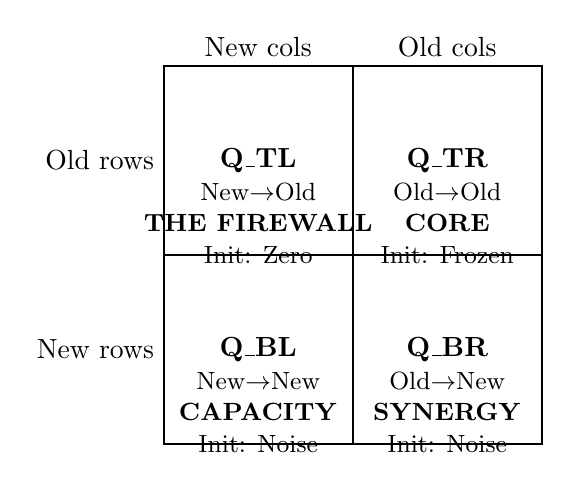
\begin{tikzpicture}[scale=0.8]
    % Draw the matrix
    \draw[thick] (0,0) rectangle (6,6);
    \draw[thick] (3,0) -- (3,6);
    \draw[thick] (0,3) -- (6,3);
    
    % Labels
    \node at (1.5,4.5) {\textbf{Q\_TL}};
    \node at (1.5,4.0) {\small New$\to$Old};
    \node at (1.5,3.5) {\small \textbf{THE FIREWALL}};
    \node at (1.5,3.0) {\small Init: Zero};
    
    \node at (4.5,4.5) {\textbf{Q\_TR}};
    \node at (4.5,4.0) {\small Old$\to$Old};
    \node at (4.5,3.5) {\small \textbf{CORE}};
    \node at (4.5,3.0) {\small Init: Frozen};
    
    \node at (1.5,1.5) {\textbf{Q\_BL}};
    \node at (1.5,1.0) {\small New$\to$New};
    \node at (1.5,0.5) {\small \textbf{CAPACITY}};
    \node at (1.5,0.0) {\small Init: Noise};
    
    \node at (4.5,1.5) {\textbf{Q\_BR}};
    \node at (4.5,1.0) {\small Old$\to$New};
    \node at (4.5,0.5) {\small \textbf{SYNERGY}};
    \node at (4.5,0.0) {\small Init: Noise};
    
    % Dimension labels
    \node[above] at (1.5,6) {New cols};
    \node[above] at (4.5,6) {Old cols};
    \node[left] at (0,4.5) {Old rows};
    \node[left] at (0,1.5) {New rows};
\end{tikzpicture}
\caption{The Directed Synergy Topology. Note the distinct initialization policies.}
\end{figure}

\subsection{Quadrant Policies}

\subsubsection{1. Core ($Q_{TR}$)}
\textbf{Role:} Preserves existing competence.
\textbf{Policy:} Frozen. Masks are set to blocking.

\subsubsection{2. Synergy ($Q_{BR}$)}
\textbf{Role:} Allows the new task to "stand on the shoulders of giants" by reading pre-trained features.
\textbf{Policy:} \textbf{Open}. We explicitly disable cross-term isolation here.
\textbf{Init:} Standard initialization ($\mathcal{N}(0, 0.02)$) to ensure gradients flow immediately.

\subsubsection{3. Capacity ($Q_{BL}$)}
\textbf{Role:} Learning strictly new features.
\textbf{Policy:} Trainable.
\textbf{Init:} Standard initialization.

\subsubsection{4. The Firewall ($Q_{TL}$)}
\textbf{Role:} The danger zone. Maps new (unstable) features to old (frozen) outputs.
\textbf{Policy:} \textbf{Zero Initialization}.
\textbf{Mechanism:} Unlike other quadrants, $W_{TL}$ is initialized to strict zeros ($0.0$). This ensures that even if the gate opens, the output contribution is zero:
\begin{equation}
    y_{old} = y_{core} + \text{Gate} \cdot 0.0 \cdot x_{new} = y_{core}
\end{equation}
This mathematically guarantees \textbf{Identity Preservation} at initialization ($t=0$). The gate can learn to open later only if it reduces loss, but it starts as a perfect firewall.

\subsection{Latent Trainability: Resolving the Gradient Paradox}

A closed gate ($G_{fwd} \approx 0$) appears to freeze its associated weights, since:
\begin{equation}
    \nabla W = \frac{\partial \mathcal{L}}{\partial y} \cdot G_{fwd} \cdot x \approx 0
\end{equation}
This creates an apparent paradox: how can a weight be "trainable" if its gradient is zero?

\textbf{Resolution:} We distinguish between \textbf{Weight Gradients} and \textbf{Gate Gradients}:

\begin{enumerate}
    \item \textbf{Weight ($W$)}: If $G_{fwd} \approx 0$, then $\nabla W \approx 0$. The weight is effectively \textbf{frozen}.
    
    \item \textbf{Gate ($G$)}: The Gate's gradient is computed independently:
    \begin{equation}
        \nabla G = \frac{\partial \mathcal{L}}{\partial y} \cdot W \cdot x
    \end{equation}
    If $W \neq 0$ (e.g., noise-initialized for $Q_{BR}$, $Q_{BL}$), then $\nabla G \neq 0$, allowing the gate to learn.
\end{enumerate}

\textbf{The Rescue Mechanism} (applied only to Gates):
\begin{equation}
    \nabla G \leftarrow \nabla G \times \text{RescueScale}
\end{equation}
where RescueScale $\approx 10^4$ compensates for the suppressed gradient magnitude.

\textbf{Key Insight:} "If the Gate is closed, the Weight is dead. But the Gate is \textit{alive and searching}. When Rescue boosts the Gate open ($G_{fwd} > 0$), the Weight begins to receive gradients and learns."

This clarifies that \textbf{Latent Trainability} refers to the Gate's ability to activate dormant weights, not to the weights themselves being trainable while silent.

\section{The Failure of Gradient Rescue (V6)}

Prior to Directed Synergy, we attempted to use "Gradient Rescue" to force gates open. This failed due to the "Double Zero" problem.
\begin{equation}
    \nabla \text{Gate} \propto \text{Weight} \times \text{Input}
\end{equation}
If weights are Zero (for stability) and Gates are Closed, the gradient is Zero.
Rescue boosts ($10000 \times$) applied to Zero are still Zero.
Using RBF routers exacerbated this, as their gradients vanish rapidly far from centroids.
\textbf{Conclusion:} Topological solutions (Directed Synergy) are superior to optimization hacks (Rescue).

\section{Experimental Results}

We evaluated Directed Synergy on the "Count Up" (Task A) $\to$ "Count Down" (Task B) chain.

\subsection{Phase 2 Results: The "Blind Router" Leak}
Initial experiments used Noise Init ($\mathcal{N}(0, 0.02)$) for both $Q_{BR}$ and $Q_{TL}$.
\begin{itemize}
    \item \textbf{Plasticity}: \textbf{Success} (Loss 0.66). The open Synergy channel allowed Task B to learn instantly.
    \item \textbf{Stability}: \textbf{Failure} (Probe Loss 17.0). The random noise in $Q_{TL}$ leaked into Task A outputs.
\end{itemize}

\subsection{Phase 3 Strategy: The Firewall}
By applying the asymmetric "Firewall" policy (Zero Init for $Q_{TL}$ only), we predict:
\begin{itemize}
    \item \textbf{Plasticity}: Remains High (Synergy channel untouched).
    \item \textbf{Stability}: Recovered (Firewall blocks noise).
\end{itemize}

\section{Conclusion}

DGE V1.1 shifts the focus from "Separation" to "Directed Synergy". By acknowledging that not all cross-terms are equal, we can design topologies that foster transfer learning (Old$\to$New) while preventing interference (New$\to$Old). The combination of asymmetric topology and selective Zero Initialization offers a mathematically sound path to continual learning.

\bibliographystyle{plain}
\begin{thebibliography}{9}
\bibitem{gge} Jansen, S. (2024). Gated Ghost Expansion.
\end{thebibliography}

\end{document}
